\begin{problem}%
{<<Колесо фортуны>>}%
{\textsl{стандартный ввод}}%
{\textsl{стандартный вывод}}%
{1 секунда}%
{64 мегабайта}{}

Развлекательный телеканал транслирует шоу «Колесо Фортуны». В процессе игры участники шоу крутят большое колесо, разделенное на сектора. В каждом секторе этого колеса записано число. После того как колесо останавливается, специальная стрелка указывает на один из секторов. Число в этом секторе определяет выигрыш игрока.\\

Юный участник шоу заметил, что колесо в процессе вращения замедляется из-за того, что стрелка задевает за выступы на колесе, находящиеся между секторами. Если колесо вращается с угловой скоростью $v$ градусов в секунду, и стрелка, переходя из сектора $X$ к следующему сектору, задевает за очередной выступ, то текущая угловая скорость движения колеса уменьшается на $k$ градусов в секунду. При этом если $v \le k$ , то колесо не может преодолеть препятствие и останавливается. Стрелка в этом случае будет указывать на сектор $X$.\\

\begin{center}
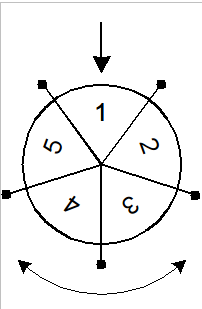
\includegraphics[scale=0.5]{images/1.png}
\end{center}

Юный участник шоу собирается вращать колесо. Зная порядок секторов на колесе, он хочет заставить колесо вращаться с такой начальной скоростью, чтобы после остановки колеса стрелка указала на как можно большее число. Колесо можно вращать в любом направлении и придавать ему начальную угловую скорость от $a$ до $b$ градусов в секунду.\\

Требуется написать программу, которая по заданному расположению чисел в секторах, минимальной и максимальной начальной угловой скорости вращения колеса и величине замедления колеса при переходе через границу секторов вычисляет максимальный выигрыш.

\InputFile

Первая строка входного файла содержит целое число $n$ — количество секторов колеса ($3 \le n \le 100$).\\

Вторая строка входного файла содержит n положительных целых чисел, каждое из которых не превышает 1000 — числа, записанные в секторах колеса. Числа приведены в порядке следования секторов по часовой стрелке. Изначально стрелка указывает на первое число.\\

Третья строка содержит три целых числа: $a$, $b$ и $k$ ($1 \le a \le b \le 10^9$, $1 \le k \le 10^9$).

\OutputFile

В выходном файле должно содержаться одно целое число — максимальный выигрыш.

\Examples

\begin{example}
\exmp{
5
1 2 3 4 5
3 5 2
}{%
5
}%
\exmp{
5
1 2 3 4 5
15 15 2
}{%
4
}%
\exmp{
5
5 4 3 2 1
2 5 2
}{%
5
}%
\end{example}

\Explanation

В первом примере возможны следующие варианты: можно придать начальную скорость колесу равную 3 или 4, что приведет к тому, что стрелка преодолеет одну границу между секторами, или придать начальную скорость равную 5, что позволит стрелке преодолеть 2 границы между секторами. В первом варианте, если закрутить колесо в одну сторону, то выигрыш получится равным 2, а если закрутить его в противоположную сторону, то — 5. Во втором варианте, если закрутить колесо в одну сторону, то выигрыш будет равным 3, а если в другую сторону, то — 4.\\

Во втором примере возможна только одна начальная скорость вращения колеса — 15 градусов в секунду. В этом случае при вращении колеса стрелка преодолеет семь границ между секторами. Тогда если его закрутить в одном направлении, то выигрыш составит 4, а если в противоположном направлении, то — 3.\\

Наконец, в третьем примере оптимальная начальная скорость вращения колеса равна 2 градусам в секунду. В этом случае стрелка вообще не сможет преодолеть границу между секторами, и выигрыш будет равен 5.

\end{problem}